\section{Лады? Лады}
\label{ch:harmony:lad}

\begin{Definition}[Лад]
    \emph{Лад}\footnote{На английском \emph{лад} --- \emph{mode}. Режим работы, способ, вид, метод} --- это интервальный шаблон, позволяющий из 12-и последовательных музыкальных звуков октавы выбрать \emph{условно} <<правильные>>. 
\end{Definition}

Если это определение показалось вам тяжеловатым, почитайте учебники или Википедию. От некоторых определений веет такой суровой философией, что хочется курить в глубокий затяг. 

Задача лада: из 12 музыкальных звуков, составляющих октаву, выбрать лишь несколько таких, которые можно играть в любом порядке и все равно будет МУЗЫКА! Задача не из тривиальных и кажется весьма субъективной, ведь всегда найдется кто-то, кто скажет: <<А мне не нравится!>>. 

Однако эта задача была решена\footnote{Не исключено, что кем-то она решается и в данный момент} предками неоднократно, и в культурном наследнии мы имеем немало ладов, самыми известными из которых являются \emph{мажорный} и \emph{минорный}.

Мажорный и минорный лады --- лады \emph{семиступенные}. То есть такой лад выбирает из 12 звуков октавы только 7.

\paragraph{Мажорный лад.} Начнем с мажорного лада, интервальная структура которого приведена на рисунке \ref{fig:harmony:lad:mode:maj}. Тёмными кружками обозначены <<выбранные>> ладом звуки --- \emph{ступени} лада. Например, вторая ступень мажорного лада находится на расстоянии 2-х полутонов от первой. Интервалы (в полутонах) между ступенями \emph{мажорного} лада расположены так:

\[
    \texttt{2-2-1-2-2-2-1}
\]

Всем с детства знакомое ДО, РЕ, МИ, ФА, СОЛЬ, ЛЯ, СИ есть не что иное, как 7 идеальных ноток, отобранных мажорным ладом, начиная от ноты ДО. Проверьте: (ДО-РЕ)=2 полутона, (РЕ-МИ)=2, (МИ-ФА)=1, (ФА-СОЛЬ)=2 и т.д. 

Интересно то, что уникальные имена получили только 7 нот, а остальные 5 нот октавы имеют производные имена (с суффиксом <<бемоль>> или <<диез>>) --- есть следствие использования ладов.

\begin{figure}[!ht]
    \centering
    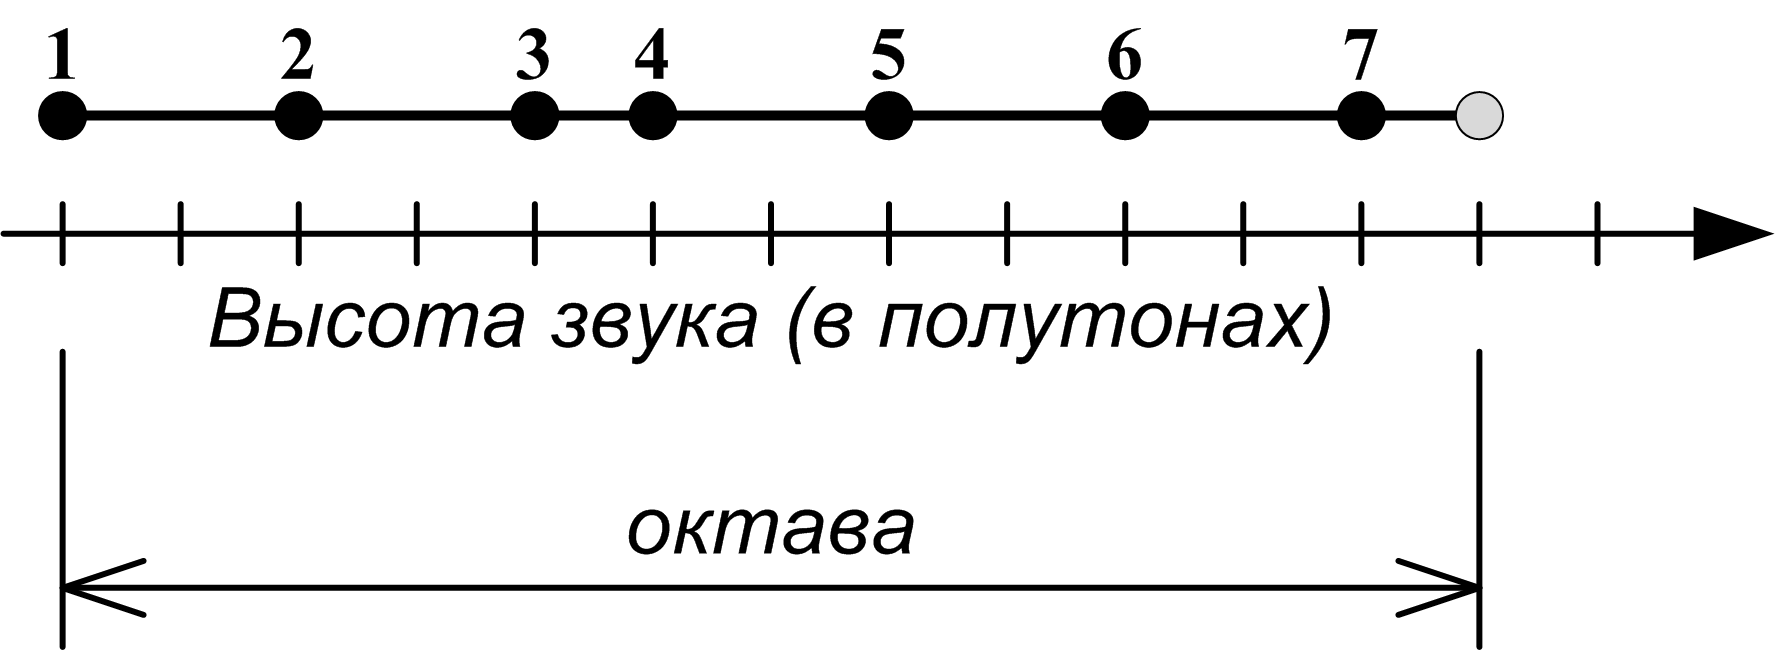
\includegraphics{fig/intervals/mode-maj} 
    \caption{Интервальная структура мажорного лада}\label{fig:harmony:lad:mode:maj}
\end{figure} 

Таким образом, шаблон лада может накладываться на любую ноту, любой музыкальный звук. Сплошная теория относительности!

Когда первая ступень лада накладывается на определенную ноту, то набор нот, попавших на ступени лада, образует \emph{тональность}\footnote{На английском \emph{тональность} --- tonality}. Допустим, мы совместили первую ступень мажорного лада с нотой ДО, тогда мы получим тональность <<ДО-мажор>>: 
\[
    \text{ДО}\xrightarrow{2}
    \text{РЕ}\xrightarrow{2}
    \text{МИ}\xrightarrow{1}
    \text{ФА}\xrightarrow{2}
    \text{СОЛЬ}\xrightarrow{2}
    \text{ЛЯ}\xrightarrow{2}
    \text{СИ}\xrightarrow{1}
\]

Базовая нота, т.е. нота, на которую наложили перую ступень лада, называется \emph{тоникой}\footnote{Ступени мажорного и минорного ладов так часто используются в теории музыки, что получили собственные названия. Нам, чтобы разобраться, достаточно запомнить, что нота, попавшая в первую ступень называется \emph{тоника}. А для общего развития: 5-я ступень --- доминанта, 4-я --- субдоминанта, 3-я --- медианта. Повторюсь: это названия ступеней как мажорного, так и минорного ладов}.

Название тональности складывается из названия ноты, попавшей на первую ступень (\emph{тоники}) и названия лада. Обычно мелодия составляется только из семи нот, входящих в тональность. Так и говорят, например, мелодия в тональности <<ЛЯ-минор>>.

\begin{Example}[Тональность <<РЕ-мажор>>]
    \label{ex:harmony:lad:d:maj}
    
    Чтобы получить ноты в тональности РЕ-мажор, нам нужно совместить ноту РЕ и первую ступень мажорного лада. Отступаем два полутона, и на вторую ступень попадет нота МИ. На третью --- ФА-диез.
    
    Целиком:
    \[
        \text{РЕ}\xrightarrow{2} 
        \text{МИ}\xrightarrow{2} 
        \text{ФА-диез}\xrightarrow{1} 
        \text{СОЛЬ}\xrightarrow{2} 
        \text{ЛЯ}\xrightarrow{2} 
        \text{СИ}\xrightarrow{2} 
        \text{ДО-диез}\xrightarrow{1}
    \]
    
    В эту тональность попали нотки, имеющие производные названия: ФА-диез, ДО-диез.
\end{Example}

Задача определить ноты, входящие в ту или иную тональность, а также количество диезов и бемолей, является любимой пыткой среди музыкальных инквизиторов. Сдвинуть шаблончик --- дело плёвое. А вот ноты после этого назвать --- уже подвиг! Совершенно искусственная проблема, растущая только от принятого способа обозначать ноты.

Например, для певца, поющего по нотам\footnote{Да, есть люди которые могут делать такие штуки со своим голосом: тянуть гласные с нужной частотой основного тона} чтобы перейти из тональности <<ДО-мажор>> в <<РЕ-мажор>> достаточно каждую исходную нотку спеть двумя полутонами выше (сдвинуть шаблон) и не думать о том, какая нота получается в итоге (закодировать название ноты).

Характерная ситуация в музыке: с практической точки зрения все оказывается проще, чем с теоретической!

Чтобы сыграть \emph{гамму}\footnote{Слово \emph{гамма} в русском очень похоже на \emph{Game} (игра) в английском. И вроде бы логично: гамма --- это то, что \emph{играется}! Но \emph{гамма} на английском --- \emph{scale}. Шкала, звукоряд} в заданной тональности нужно:
\begin{itemize}
    \item начать с ноты первой ступени;
    \item продолжить играть ноты тональности в порядке возрастания (или убывания) высоты;
    \item сыграв таким образом одну или несколько октав, закончить на ноте первой ступени (естественно уже в другой октаве); 
    \item (необязательно) проиграть только что сыгранную последовательность в обратном порядке.
\end{itemize}

Например, гамма в тональности <<ДО-мажор>> или просто <<гамма ДО-мажор>> это известное: 
\begin{center}
    ДО, РЕ, МИ, ФА, СОЛЬ, ЛЯ, СИ, ДО, СИ, ЛЯ, СОЛЬ, ФА, МИ, РЕ, ДО.
\end{center}


\paragraph{Минорный лад.} Интервальная структура \emph{минорного} лада приведена на рисунке \ref{fig:harmony:lad:mode:min}. Интервалы (в полутонах) между ступенями \emph{минорного} лада расположены так:
\[
    \texttt{2-1-2-2-1-2-2}
\]

\begin{figure}[!ht]
    \centering
    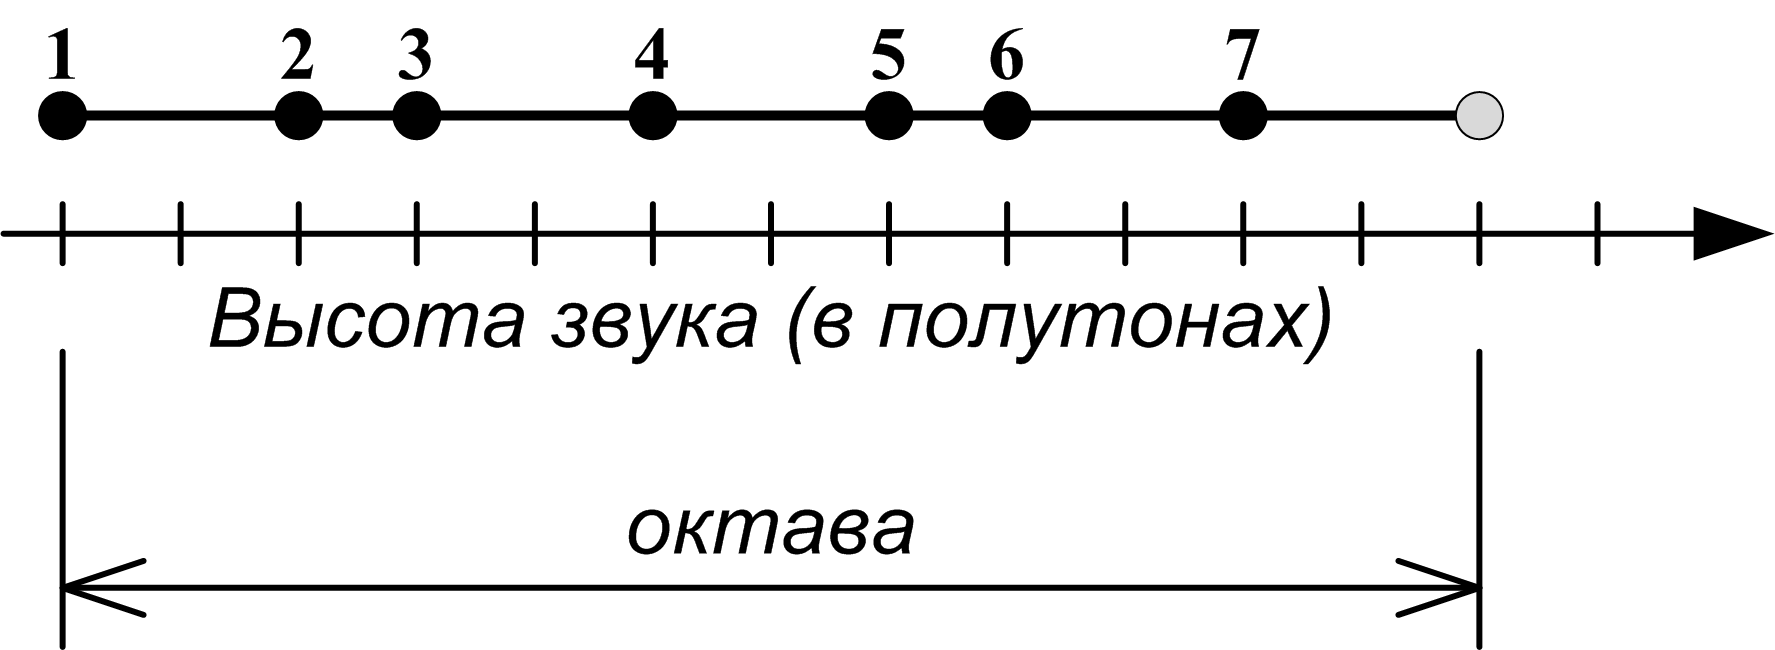
\includegraphics{fig/intervals/mode-min} 
    \caption{Интервальная структура минорного лада}\label{fig:harmony:lad:mode:min}
\end{figure} 

Заметьте, что если замкнуть минорную интервальную структуру в кольцо и немного повращать (а это можно сделать, так как в следующей октаве все повторится), то получится мажорный лад. Совместите первую ступень мажорного лада и третью минорного и убедитесь, что в принципе структура этих ладов одна и та же. 

Например, давайте положим в первую ступень минора ноту ЛЯ. Получим тональность, состоящую из нот:
\begin{center}
    ЛЯ, СИ, ДО, РЕ, МИ, ФА, СОЛЬ.
\end{center}

Названия нот в тональности <<ЛЯ-минор>> те же, что и в <<ДО-мажор>> (как видно, нет ни одной нотки с бемолем или диезом). Поэтому тональности <<ДО-мажор>> и <<ЛЯ-минор>> называются \emph{параллельными}. Как нетрудно догадаться, параллельных тональностей столько же, сколько нот в октаве: 12. А вот \emph{гамму} <<ЛЯ-минор>>:
\begin{center}
    ЛЯ, СИ, ДО, РЕ, МИ, ФА, СОЛЬ, ЛЯ, СОЛЬ, ФА, МИ, РЕ, ДО, СИ, ЛЯ
\end{center}
с гаммой <<ДО-мажор>> точно на слух не спутаешь!

\paragraph{Современные 7-ступенные лады.} Эти лады имеют сходную интервальную структуру и называются диатоническими\footnote{Диатонические лады или просто <<диатоника>> --- это система семиступенных ладов, постоенных из пяти интервалов величиной в два полутона, и двух полутоновых интервалов. $5\cdot2 + 2\cdot 1 = 12$ --- октава}. Мажор и минор --- также диатонические лады. На рисунке \ref{fig:harmony:lad:modes} иображена октава, разделенная на 12 полутонов. Лады отличаются друг от друга только тем, откуда начинается первая ступень. Каждый из семи возможных вариантов имеет собственное название. 

Например, первая ступень <<Лидийского>> лада начинается с 4-й отметки на октаве, и, обойдя от 4-й отметки всю окраву, легко получить его интервальную структуру:
\[
    \texttt{2-2-2-1-2-2-1}
\]

\begin{figure}[!ht]
    \centering
    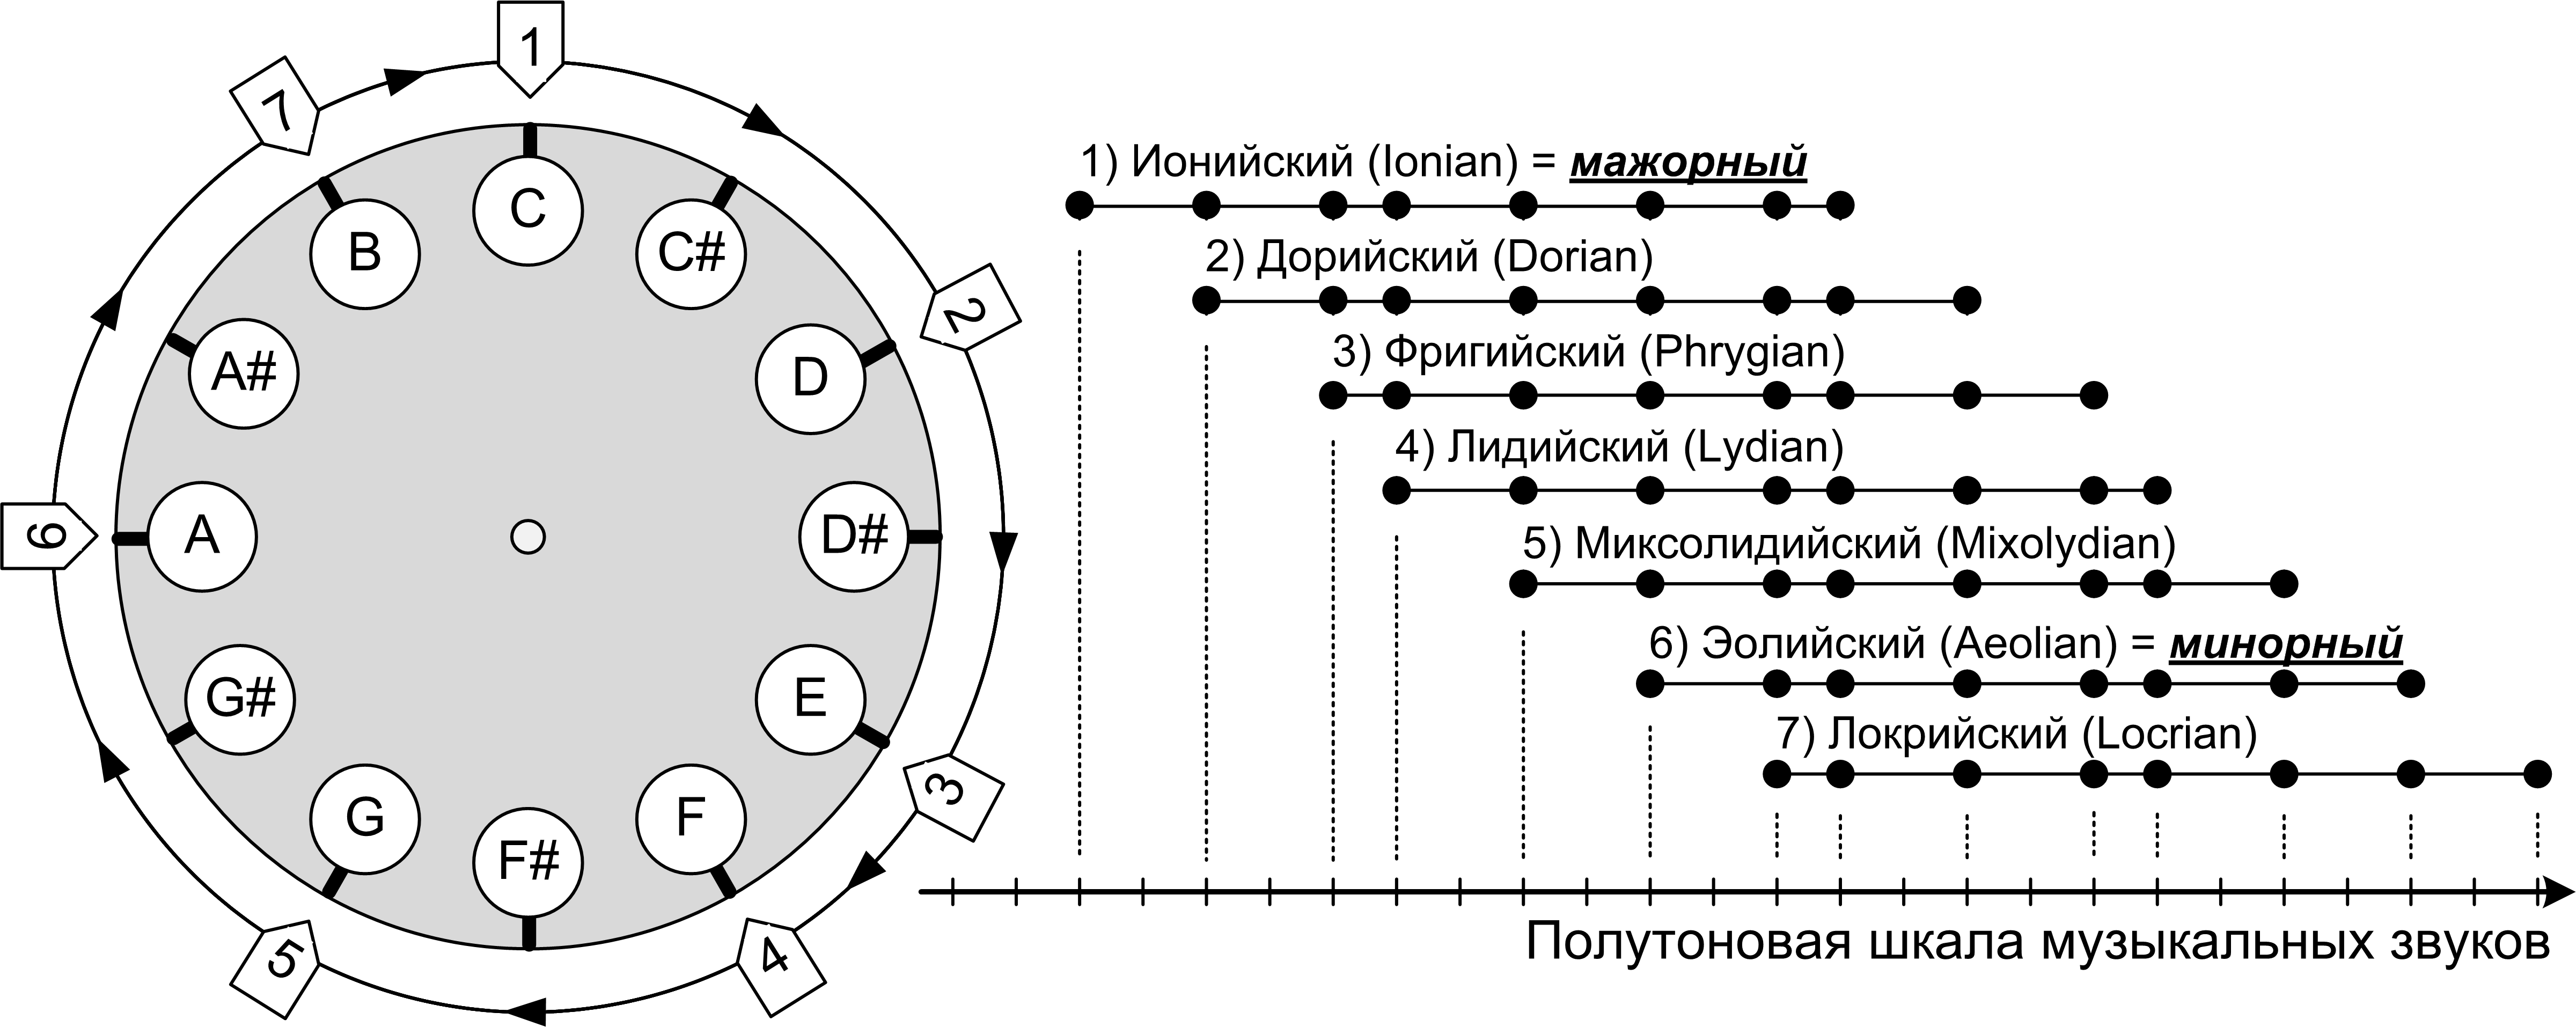
\includegraphics[width=\textwidth]{fig/intervals/modes} 
    \caption{Интервальная структура диатонических ладов}\label{fig:harmony:lad:modes}
\end{figure} 

<<Лидийский>> лад активно используется в джазовой музыке. Если вы хотите послушать <<ФА-лидийскую>> гамму, то достаточно сыграть:
\begin{center}
    ФА, СОЛЬ, ЛЯ, СИ, ДО, РЕ, МИ, ФА, МИ, РЕ, ДО, СИ, ЛЯ, СОЛЬ, ФА
\end{center}

То же самое в латинских обозначениях нот:
\begin{center}
    F, G, A, B, C, D, E, F, E, D, C, B, A, G, F
\end{center}
 
Построенная от ноты ФА(F), <<ФА-лидийская>> тональность содержит (как видно из рисунка \ref{fig:harmony:lad:modes}) ноты без диезов и бемолей. Кстати, этот лад для мелодий, дарящих ощущение счастья.


\paragraph{Пентатоника.} Пентатоника --- это тоже лад, но имеющий только 5-ступеней. То есть пентатоника из 12 нот октавы выделяет только 5 <<правильных>>, из которых можно составлять мелодию. Аналогично 7-ступенным ладам, получают 5 вариантов ладов с различными названиями, см. рисунок \ref{fig:harmony:lad:pentatonic}.

\begin{figure}[!ht]
    \centering
    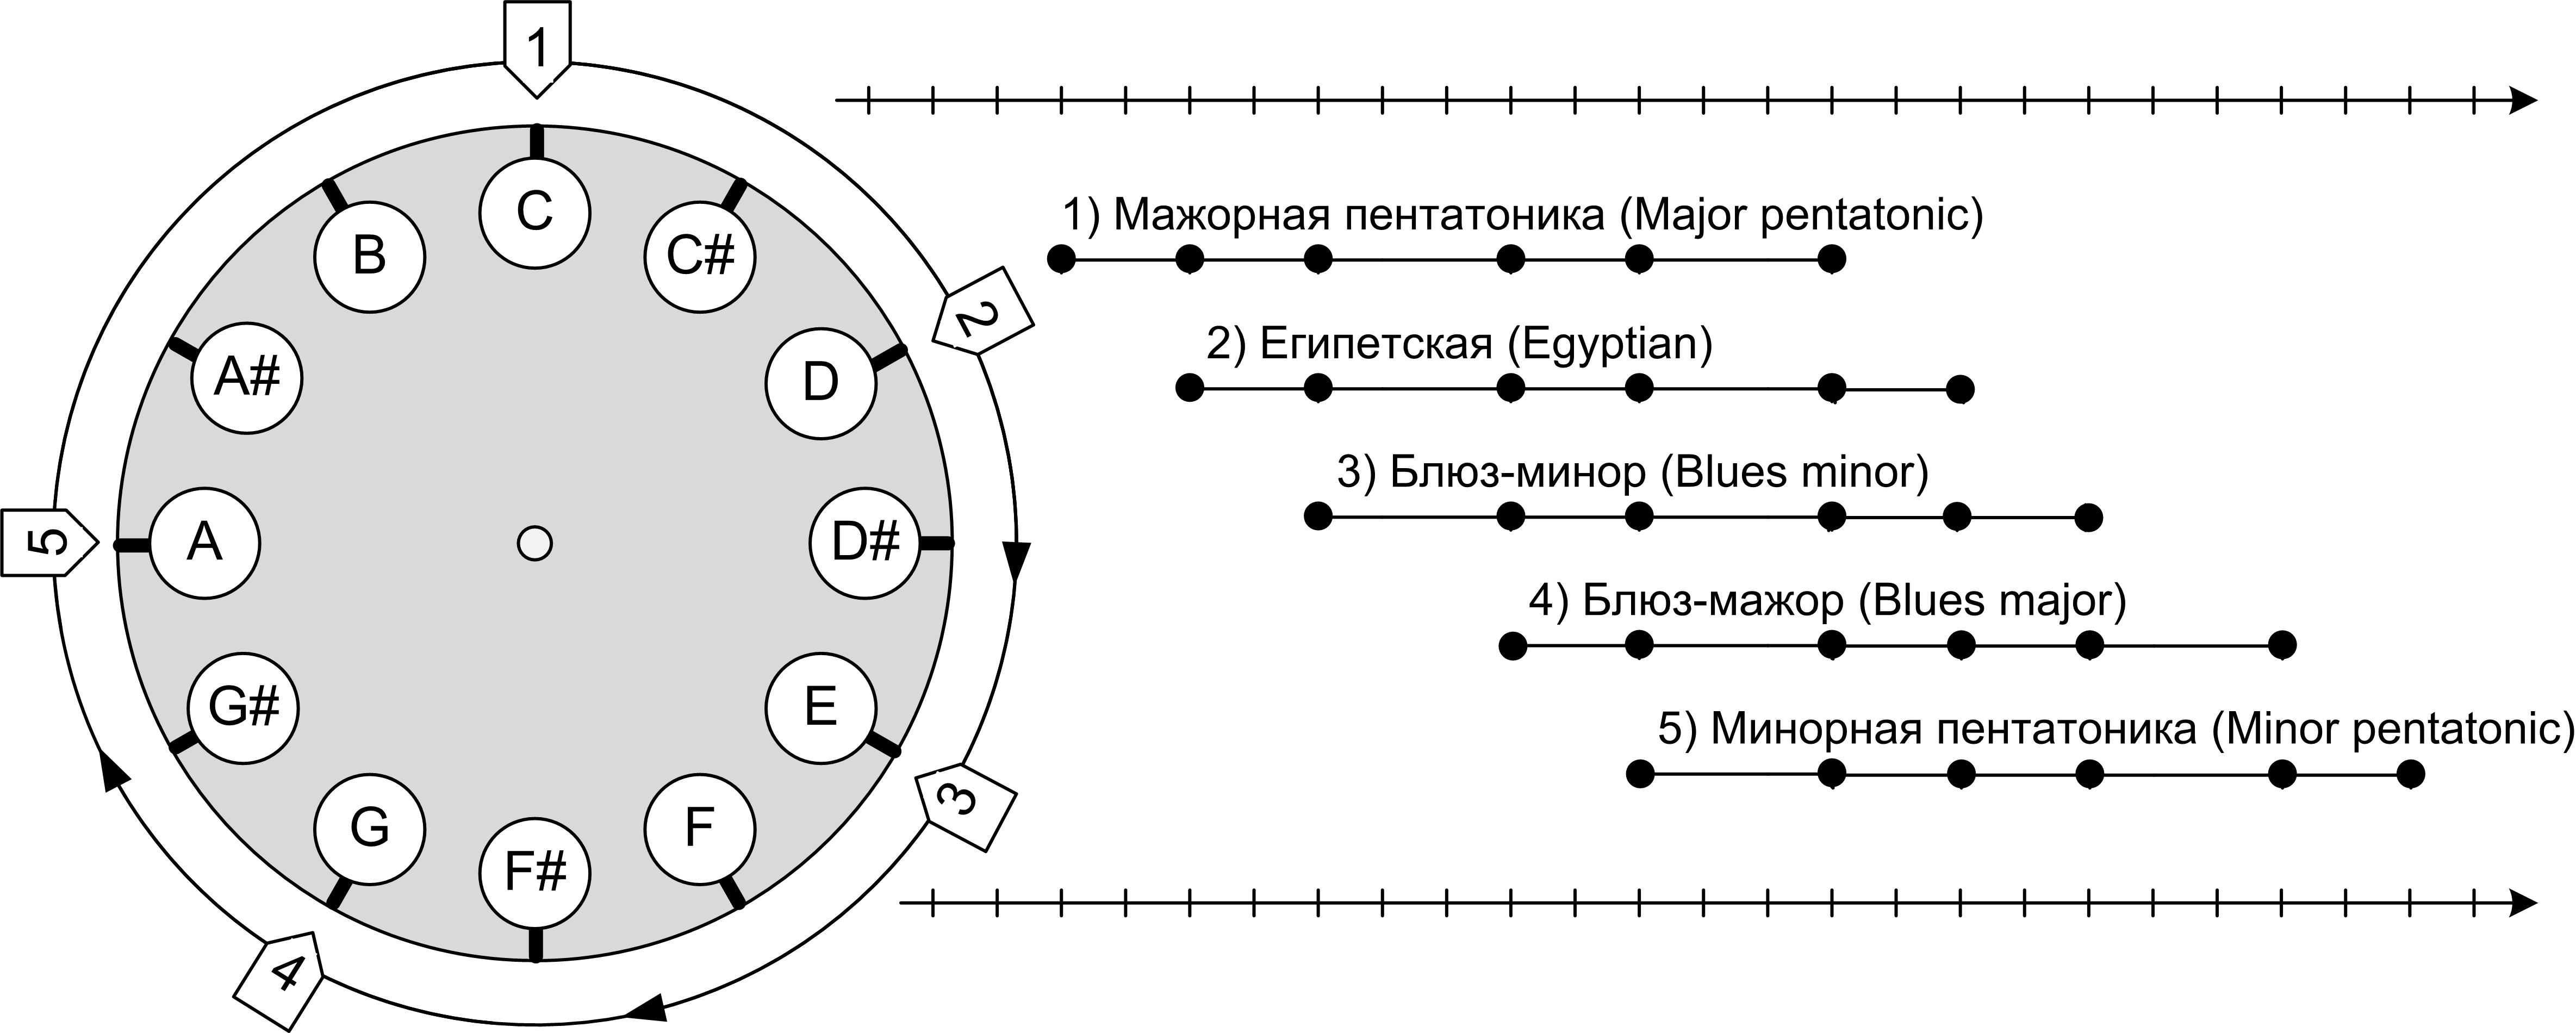
\includegraphics[width=\textwidth]{fig/intervals/pentatonic} 
    \caption{Интервальная структура пентатоники}\label{fig:harmony:lad:pentatonic}
\end{figure} 

Соответственно, например, интервальная структура мажорной пентатоники в полутонах:
\[
    \texttt{2-2-3-2-3}
\]

Обратите внимание, что пять ступеней пентатоники полностью содержатся в семиступенной структуре. Сравните рисунки \ref{fig:harmony:lad:pentatonic} и \ref{fig:harmony:lad:modes} и убедитесь, что пентатонику из диатоники можно получить, <<выкинув>> 4-ю и 7-ю отметки на октаве диатонических ладов.


%TODO: гамма лада в основных нотах
